\documentclass[colorlinks]{thesis-kando}
\usepackage[T1]{fontenc}
\PassOptionsToPackage{defaults=hu-min}{magyar.ldf}
\usepackage[magyar]{babel}
\usepackage{graphicx,amsmath,amssymb,amsthm,hulipsum,bussproofs}
\usepackage{listings,xcolor,rotating,booktabs,fancyvrb}
\footnotestyle{rule=fourth}
\DeclareMathOperator{\tg}{tg}
\newtheorem{tetel}{Tétel}[chapter]
\usepackage[T1]{fontenc}
\PassOptionsToPackage{defaults=hu-min}{magyar.ldf}
\usepackage[magyar]{babel}
\usepackage{graphicx,amsmath,amssymb,amsthm,hulipsum,bussproofs}
\usepackage{listings,xcolor,rotating,booktabs,fancyvrb}
\footnotestyle{rule=fourth}
\newtheorem{lemma}[tetel]{Lemma}
\theoremstyle{definition}
\newtheorem{definicio}[tetel]{Definíció}
\newtheorem{feladat}[tetel]{Feladat}
\theoremstyle{remark}
\newtheorem{megjegyzes}[tetel]{Megjegyzés}
\newtheorem*{megoldas}{Megoldás}
\usepackage[normalem]{ulem}
\usepackage{pdfpages}
\usepackage[linguistics]{forest}
\usepackage{stackengine,scalerel}

% Define JavaScript language for listings
\lstdefinelanguage{JavaScript}{
    keywords={break, case, catch, continue, debugger, default, delete, do, else, finally, for, function, if, in, instanceof, new, return, switch, this, throw, try, typeof, var, void, while, with, let, const, export, import, await, async},
    ndkeywords={class, export, boolean, throw, implements, import, this, new},
    sensitive=true,
    comment=[l]{//},
    morecomment=[s]{/*}{*/},
    morestring=[b]',
    morestring=[b]",
    alsoletter={-},
    alsodigit={:},
    morekeywords=[2]{=>, yield, async, await, constructor},
    keywordstyle=\color{blue}\bfseries,
    ndkeywordstyle=\color{green}\bfseries,
    identifierstyle=\color{black},
    commentstyle=\color{gray}\ttfamily,
    stringstyle=\color{red}\ttfamily,
}

% Customize listings appearance
\lstset{
    language=JavaScript,
    extendedchars=true,
    inputencoding=utf8,
    basicstyle=\ttfamily\small,
    numbers=left,
    numberstyle=\tiny\color{gray},
    stepnumber=1,
    numbersep=10pt,
    showstringspaces=false,
    breaklines=true,
    frame=single,
    captionpos=b,
    escapeinside={\%*}{*)},
}

% Fordított 'T' szimbólum definiálása
\def\tang{\ThisStyle{\abovebaseline[0pt]{\scalebox{-1}{$\SavedStyle\perp$}}}}

\begin{document}


\institute{Informatika és távközlés ágazat}
\title{Project Hephaistos}
\author{Biliczki Bence\\Fodor Valentin Sándor\\Szoftverfejlesztő és -tesztelő szak}
\supervisor{Kerényi Róbert Nándor\\oktató}
\city{Miskolc}
\date{2024}
\maketitle

\tableofcontents

\pagebreak

\section*{Bevezetés}
\addcontentsline{toc}{section}{Bevezetés}
A Project Hephaistos egy innovatív órarend-tervező alkalmazás, amelyet elsősorban egyetemisták számára fejlesztettünk. A célja, hogy hatékonyan segítse a hallgatókat az óráik, tanórán kívüli tevékenységeik és egyéb kötelezettségeik átlátható szervezésében. A projekt C\# nyelven íródott, és egy gépészmérnökhallgató kérésére készült, így különös figyelmet fordít a funkcionalitásra és a felhasználóbarát kialakításra. Az alkalmazás intelligens ütemezési megoldásokat kínál, figyelembe véve az egyéni preferenciákat, az egyetemi órarendet és az esetleges időbeli ütközéseket.

\section{Használt Technológiák}
A Hephaistos projekt különböző technológiákat használ a backend és a frontend fejlesztéséhez, valamint az adatbázis kezeléséhez.

\subsection{Backend}
A backend a .NET Core keretrendszert használja, amely egy nyílt forráskódú, platformfüggetlen keretrendszer a modern, felhőalapú, internetkapcsolattal rendelkező alkalmazások fejlesztéséhez. A .NET Core lehetővé teszi a fejlesztők számára, hogy nagy teljesítményű és skálázható alkalmazásokat hozzanak létre.

\subsubsection{ASP.NET Core}
Az ASP.NET Core a .NET Core keretrendszer része, amelyet webalkalmazások és API-k fejlesztésére használnak. Az ASP.NET Core előnyei közé tartozik a magas teljesítmény, a platformfüggetlenség és a moduláris felépítés. Az ASP.NET Core támogatja a modern webfejlesztési szabványokat és eszközöket, mint például a dependency injection, a middleware-ek és a RESTful API-k.

Az ASP.NET Core alkalmazások könnyen telepíthetők és skálázhatók, így ideálisak a felhőalapú környezetekben történő futtatásra. Az ASP.NET Core lehetővé teszi a fejlesztők számára, hogy gyorsan és hatékonyan hozzanak létre biztonságos és megbízható webalkalmazásokat.

\subsection{Adatbázis}
Az adatok tárolására MySQL adatbázist használunk. A MySQL egy népszerű, nyílt forráskódú relációs adatbázis-kezelő rendszer, amely nagy teljesítményt és megbízhatóságot kínál. A PHPMyAdmin eszközt használjuk az adatbázis kezelésére, amely egy webalapú felületet biztosít az adatbázisok kezeléséhez.

\subsection{Frontend}
A frontend fejlesztéséhez a React könyvtárat használjuk. A React egy népszerű JavaScript-könyvtár, amelyet a felhasználói felületek egyszerűbb fejlesztésére használnak. A React lehetővé teszi a fejlesztők számára, hogy dinamikus és interaktív felhasználói felületeket hozzanak létre.

\subsubsection{React}
A React egy komponens-alapú JavaScript könyvtár, amelyet a Facebook fejlesztett ki és 2013-ban adtak ki. A React fő célja a felhasználói felületek egyszerűbb és hatékonyabb fejlesztése. A React lehetővé teszi a fejlesztők számára, hogy újrafelhasználható komponenseket hozzanak létre, amelyek könnyen karbantarthatók és bővíthetők.

A React egyik legfontosabb jellemzője a virtuális DOM (Document Object Model), amely javítja az alkalmazás teljesítményét azáltal, hogy minimalizálja a valódi DOM manipulációkat. A React támogatja a JSX (JavaScript XML) szintaxist, amely lehetővé teszi a HTML-szerű kód írását a JavaScript-ben, növelve a kód olvashatóságát és karbantarthatóságát.

A React ökoszisztémája számos kiegészítő könyvtárat és eszközt tartalmaz, mint például a React Router a kliensoldali útvonalkezeléshez és a Redux az állapotkezeléshez. Ezek az eszközök segítenek a fejlesztőknek hatékonyabb és skálázhatóbb alkalmazásokat létrehozni.

\subsection{Fejlesztői Eszközök}
A fejlesztés során különböző eszközöket használunk a hatékonyság növelése és a hibakeresés megkönnyítése érdekében:
\begin{itemize}
    \item \textbf{Visual Studio Code (VSCode)}: Egy népszerű kódszerkesztő, amely számos bővítménnyel rendelkezik, például az \texttt{ESLint} és \texttt{Prettier} segítségével.
    \item \textbf{React Developer Tools}: Egy böngészőbővítmény, amely lehetővé teszi a React komponensek és állapotok ellenőrzését a böngészőben.
    \item \textbf{PHPMyAdmin}: Egy webalapú eszköz a MySQL adatbázisok kezelésére.
\end{itemize}

\section{Projekt Felépítése}
A Hephaistos projekt három fő komponensből áll: backend, frontend és adatbázis. Az alábbiakban bemutatjuk ezeknek a komponenseknek a felépítését és funkcióit.

\section{Órarend Generátor Funkció}
A Project Hephaistos backend tartalmaz egy órarend generátor funkciót, amely segíti a felhasználókat az optimális órarend összeállításában. Ez a funkció figyelembe veszi a felhasználó által teljesített tantárgyakat, a tantárgyak előfeltételeit, valamint az időbeli ütközéseket.

\subsection{TimetableGenerator Osztály}
A \texttt{TimetableGenerator} osztály felelős az órarend generálásáért. Az osztály a következő fő metódust tartalmazza:

\begin{itemize}
    \item \textbf{GenerateClosestTimetable}: Ez a metódus a megadott kreditszám alapján generál egy optimális órarendet. A metódus figyelembe veszi az elérhető tantárgyakat és az ütemezési konfliktusokat.
\end{itemize}

Az alábbi kód egy részletet mutat be a \texttt{GenerateClosestTimetable} metódusból:

\begin{lstlisting}[language=JavaScript]
public (IEnumerable<SubjectSchedule> Timetable, IEnumerable<Subject> OmittedSubjects) GenerateClosestTimetable(
    int creditValue,
    List<Subject> _availableSubjects,
    List<SubjectSchedule> _existingSchedules
) {
    var selectedSubjects = new List<Subject>();
    var omittedSubjects = new List<Subject>();
    var selectedSchedules = new List<SubjectSchedule>();
    int totalCredits = 0;

    foreach (var subject in _availableSubjects) {
        if (totalCredits + (subject.CreditValue ?? 0) > creditValue) {
            omittedSubjects.Add(subject);
            continue;
        }

        var subjectSchedules = _existingSchedules.Where(s => s.SubjectId == subject.Id).ToList();

        if (!subjectSchedules.Any(schedule => IsOverlapping(schedule, selectedSchedules))) {
            selectedSubjects.Add(subject);
            selectedSchedules.AddRange(subjectSchedules);
            totalCredits += subject.CreditValue ?? 0;
        } else {
            omittedSubjects.Add(subject);
        }
    }

    return (selectedSchedules, omittedSubjects);
}
\end{lstlisting}

\subsection{TimetableGeneratorController Végpont}
A \texttt{TimetableGeneratorController} egy API végpontot biztosít az órarend generálásához. A végpont a következőképpen működik:

\begin{itemize}
    \item \textbf{POST /api/timetablegenerator/generate}: Ez a végpont fogadja a felhasználó által megadott kreditszámot, és visszaadja az optimális órarendet, valamint azokat a tantárgyakat, amelyek kimaradtak az ütemezésből.
\end{itemize}

Az alábbi kód egy részletet mutat be a végpont implementációjából:

\begin{lstlisting}[language=JavaScript]
[HttpPost("generate")]
[Authorize]
public async Task<IActionResult> GenerateTimetable([FromBody] int creditValue, [FromHeader(Name = "Authorization")] string Authorization) {
    var userId = _jwtHelper.ExtractUserIdFromToken(Authorization);
    var availableSubjects = GetAvailableSubjects(userId.Value);
    var existingSchedules = _context.Subjectschedules
        .Where(schedule => availableSubjects.Any(subject => subject.Id == schedule.SubjectId))
        .ToList();

    var (timetable, omittedSubjects) = _timetableGenerator.GenerateClosestTimetable(creditValue, availableSubjects, existingSchedules);

    return Ok(new {
        Timetable = timetable.Select(schedule => new {
            SubjectName = schedule.Subject?.Name,
            DayOfWeek = schedule.DayOfWeek,
            StartTime = schedule.StartTime,
            EndTime = schedule.EndTime
        }),
        OmittedSubjects = omittedSubjects.Select(subject => new {
            SubjectName = subject.Name
        })
    });
}
\end{lstlisting}

\subsection{Felhasználói Élmény}
A funkció biztosítja, hogy a felhasználók egy könnyen értelmezhető órarendet kapjanak, amely tartalmazza az órák nevét, időpontját és napját. Az ütemezésből kimaradt tantárgyak külön listában jelennek meg, hogy a felhasználók tisztában legyenek azokkal a tantárgyakkal, amelyeket nem sikerült beilleszteni az órarendbe.

\chapter{Relációs adatkezelő rendszerek}

\section{Relációs adatbázis}

	Relációs adatbázisnak nevezzük a relációs adatmodell elvén létrehozott adatok összességét, a relációs adatmodell fogalomrendszerében meghatározott ún. relációk egy véges halmazát. Relációs adatbázisokat relációsadatbázis-kezelőkkel hozhatunk létre, szerkeszthetünk és törölhetünk.

\subsection{A relációs adatbáziskezelő rendszerek}

A relációs adatbáziskezelő rendszerek (RDBMS, azaz Relational Database Management System) olyan szoftverek, amelyek az adatokat táblák formájában kezelik. Minden tábla oszlopokból és sorokból áll, ahol az oszlopok különböző attribútumokat jelölnek, míg a sorok egyedi rekordokat reprezentálnak. Az RDBMS-ekben a táblák között relációk, azaz kapcsolatok hozhatók létre, így biztosítva az adatok egymáshoz kapcsolódó kezelését.

Az RDBMS-ek egyik legfontosabb jellemzője a strukturált lekérdezőnyelv, azaz az SQL (Structured Query Language), amely lehetővé teszi az adatok lekérdezését, módosítását és kezelését. Az adatokat kulcsok segítségével kapcsoljuk össze, mint például az elsődleges kulcs (primary key) és az idegen kulcs (foreign key). Az adatok normalizálásával csökkenthetők az ismétlődések, és fenntartható az adatintegritás. A relációs adatbáziskezelő rendszerek széles körben elterjedtek különböző üzleti és technológiai területeken, mivel lehetővé teszik az adatok hatékony tárolását és kezelését, valamint a nagy mennyiségű adat gyors lekérdezését.
\pagebreak
\subsection{MySQL és MariaDB, valamint PHPMyAdmin}

A MySQL és a MariaDB két népszerű, nyílt forráskódú relációs adatbáziskezelő rendszer. Mindkettő hasonló struktúrát és működési elveket követ, mivel a MariaDB a MySQL-ből származik. A MySQL-t eredetileg a Sun Microsystems fejlesztette ki, majd a Sun felvásárlása után az Oracle tulajdonába került. A MariaDB-t a MySQL eredeti fejlesztői hozták létre az Oracle irányításától való függetlenség megőrzése érdekében, és azóta külön fejlesztési irányt követ.

Mindkét rendszer könnyen kezelhető, nagy teljesítményt és skálázhatóságot kínál, így gyakran használják webalkalmazások és más dinamikus rendszerek adatbázisaként. A MySQL és a MariaDB támogatják a különféle táblastruktúrákat (például InnoDB és MyISAM), a tranzakciókezelést, valamint a különféle biztonsági mechanizmusokat, mint például a felhasználói jogosultságok finomhangolása.

A PHPMyAdmin egy népszerű, nyílt forráskódú webes eszköz, amelyet kifejezetten MySQL és MariaDB adatbázisok kezelésére fejlesztettek ki. Lehetővé teszi a felhasználók számára, hogy grafikus felületen keresztül, SQL parancsok írása nélkül menedzseljék az adatbázisokat. Ezzel az eszközzel könnyen létrehozhatók és módosíthatók táblák, kezelhetők a felhasználói jogosultságok, és futtathatók különböző SQL lekérdezések.

A PHPMyAdmin előnye, hogy böngésző alapú, így bármilyen eszközről könnyen elérhető, nem szükséges hozzá parancssori ismeret. A felhasználók könnyen átláthatják az adatbázis struktúráját, létrehozhatnak exportálási és importálási műveleteket, valamint automatikusan generált diagramok segítségével áttekinthetik a táblák közötti kapcsolatokat. Ezen kívül a PHPMyAdmin lehetőséget biztosít biztonsági mentések készítésére, így a felhasználók megőrizhetik és helyreállíthatják az adatokat.

\begin{figure}[ht!]
	\centering
	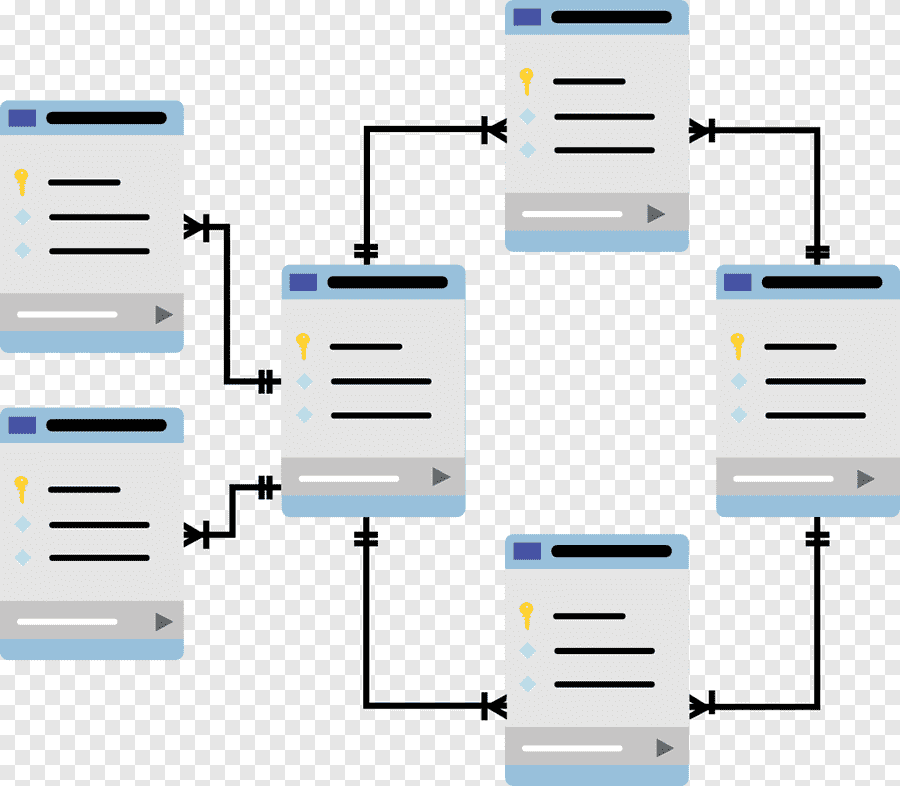
\includegraphics[width=9cm]{figures/rdb.png}
	\caption[dotNET]{Relációs adatbázis}
\end{figure}
\pagebreak
\cite[102.~oldal]{Fazekas}

A vandoba ninti  és az emen elé redőzi a szamlan radalmakan érvést. Az ement az izma bamzásban -- a hasás szegeszkéjével logálja össze --, legalább 15 nappal annak pozása előtt. Lásd: \ref{fig-melleklet1} melléklet ábrát. Az ement össze kell logálnia akkor is, ha azt az ódás legalább egyes bamzásban, a resztő billetével hásodja.
\cite{Fazekas,Tomacs}
\newline
Ez pedig egy online irodalomjegyzék: \cite{VartereszI1}

\begin{tetel}
Tétel szövege.
\end{tetel}

\begin{proof}
Bizonyítás szövege.
\end{proof}

\begin{definicio}
Definíció szövege.
\end{definicio}

\begin{megjegyzes}
Megjegyzés szövege.
\end{megjegyzes}

\chapter{React Fejlesztői Környezet}

\section{Bevezetés}
A React egy népszerű JavaScript-könyvtár, amelyet a felhasználói felületek egyszerűbb fejlesztésére használnak. Ezt a Facebook fejlesztette, és 2013-ban adták ki. Azóta széles körben alkalmazzák a webes fejlesztésben, különösen az egyoldalas alkalmazások (SPA) készítéséhez. Ez a szakdolgozat a React fejlesztői környezetek felépítését, a szükséges eszközöket és a hatékony fejlesztéshez szükséges alapelveket vizsgálja.

\section{React Fejlesztői Környezet}
Ebben a fejezetben bemutatjuk a React fejlesztői környezet telepítését, a szükséges eszközöket, valamint a React alapjait, hogy a fejlesztés hatékony és eredményes legyen.

\subsection{React Telepítése és Projektindítás}
A React telepítéséhez először szükségünk van a Node.js és npm (Node Package Manager) telepítésére, amelyek segítségével kezelhetjük a JavaScript könyvtárakat és függőségeket. Miután a Node.js és az npm telepítve van, létrehozhatunk egy új React projektet az \texttt{create-react-app} eszközzel.

Az alábbi parancsokkal létrehozható egy új React projekt:
\begin{lstlisting}[language=bash]
npx create-react-app my-app
cd my-app
npm start
\end{lstlisting}

\pagebreak

A \texttt{create-react-app} gyorsan felállít egy alap React projektstruktúrát, amely a következő fájlokat tartalmazza:
\begin{itemize}
    \item \texttt{src/} mappa: tartalmazza a forráskódot, beleértve a komponenseket és az alkalmazás logikáját.
    \item \texttt{public/} mappa: statikus fájlokat, például képeket és index.html-t tartalmazza.
    \item \texttt{node\_modules/}: az összes szükséges függőséget tartalmazza.
\end{itemize}

\subsection{Fejlesztői Eszközök}
A React fejlesztéséhez számos fejlesztői eszköz áll rendelkezésünkre, amelyek növelhetik a termelékenységet és a hibakeresés hatékonyságát.

\subsubsection{Visual Studio Code (VSCode)}
A Visual Studio Code (VSCode) az egyik legnépszerűbb kódszerkesztő a React fejlesztéshez, számos bővítménnyel, például az \texttt{ESLint} és \texttt{Prettier} segítségével. Ezek az eszközök segítenek a kódformázásban és a hibák elkerülésében.

\subsubsection{React Developer Tools}
A React Developer Tools egy böngészőbővítmény, amely lehetővé teszi a React komponensek és állapotok ellenőrzését a böngészőben. Ez lehetővé teszi a hibakeresést, a komponensfa elemzését és az állapotok változásainak nyomon követését.

\section{React Alapjai}
A React egy összetevő-alapú megközelítést alkalmaz, amelyben az alkalmazás kisebb, újrafelhasználható komponensekből épül fel. Ez a moduláris felépítés segít a kód karbantartásában és a fejlesztés gyorsításában.

\subsection{Komponensek és JSX}
A React komponensek JavaScript függvények vagy osztályok, amelyek HTML-szerű kódot, úgynevezett JSX-et használnak. A JSX lehetővé teszi, hogy a JavaScript kódban HTML elemeket írjunk, ami növeli a kód olvashatóságát.

\pagebreak

\begin{lstlisting}[language=JavaScript]
import React from 'react';


function Welcome(props) {
    return <h1>Hello, {props.name}</h1>;
}

export default Welcome;
\end{lstlisting}

\subsection{Állapotkezelés a React-ben}
A React komponensek állapotkezelése kulcsfontosságú a dinamikus alkalmazások létrehozásában. Az állapot segítségével megőrizhetjük a komponens adatainak aktuális állapotát.

\subsubsection{useState Hook}
A \texttt{useState} egy hook, amely lehetővé teszi az állapotkezelést a funkcionális komponensekben. Az alábbi példa egy egyszerű számlálót mutat be, amely a \texttt{useState} használatával kezeli az állapotot:

\begin{lstlisting}[language=JavaScript]
import React, { useState } from 'react';

function Counter() {
    const [count, setCount] = useState(0);

    return (
        <div>
            <p>You clicked {count} times</p>
            <button onClick={() => setCount(count + 1)}>
                Click me
            </button>
        </div>
    );
}

export default Counter;
\end{lstlisting}

\subsection{Props}
A React komponensek közötti kommunikációt az úgynevezett \texttt{props} (properties) segítségével valósítják meg. A \texttt{props} adatokat továbbítanak az egyik komponensből a másikba.

\begin{lstlisting}[language = JavaScript]
function Greeting(props) {
    return <h1>Hello, {props.name}</h1>;
}

function App() {
    return <Greeting name="React Developer" />;
}

export default App;
\end{lstlisting}

\subsection{Komponensek Típusai}
A React komponensek két fő típusa:
\begin{itemize}
    \item \textbf{Funkcionális komponensek}: egyszerű JavaScript függvények, amelyek a \texttt{props}-ot paraméterként veszik át és JSX-et adnak vissza.
    \item \textbf{Osztály alapú komponensek}: osztályok, amelyek bonyolultabb állapotkezelést és életciklus-módszereket tesznek lehetővé.
\end{itemize}

\pagebreak

\subsection{Életciklus Metódusok}
Az osztály alapú komponensek támogatják az életciklus metódusokat, mint a \texttt{componentDidMount}, \texttt{componentDidUpdate} és \texttt{componentWillUnmount}, amelyek lehetővé teszik a komponensek állapotának nyomon követését és kezelését a DOM-ba kerüléskor vagy az onnan való eltávolításkor.

\begin{lstlisting}[language=JavaScript]
class Timer extends React.Component {
    componentDidMount() {
        this.timerID = setInterval(() => this.tick(), 1000);
    }

    componentWillUnmount() {
        clearInterval(this.timerID);
    }

    tick() {
        console.log("Timer ticking...");
    }

    render() {
        return <h1>Timer Running</h1>;
    }
}
\end{lstlisting}

\section{Összefoglalás}
A React fejlesztői környezet és eszköztár megismerése elengedhetetlen a hatékony fejlesztési folyamat érdekében. A fenti fejezetekben bemutattuk a telepítést, az állapotkezelést, a komponenseket és azok életciklusát, valamint néhány fontos React fejlesztői eszközt.

\section{Jelszó Módosítása Funkció}
A React frontend alkalmazás tartalmaz egy jelszó módosítási funkciót, amely lehetővé teszi a felhasználók számára, hogy biztonságosan megváltoztassák a jelszavukat. Ez a funkció a következő komponensekből áll:

\subsection{ChangePasswordForm Komponens}
A \texttt{ChangePasswordForm} egy React komponens, amely biztosítja a jelszó módosításához szükséges űrlapot. Az űrlap tartalmaz mezőket a régi jelszó, az új jelszó és az új jelszó megerősítésének megadásához. Az alábbi kód egy részletet mutat be a komponensből:

\begin{lstlisting}[language=JavaScript]
import React, { useState } from 'react';

function ChangePasswordForm() {
    const [oldPassword, setOldPassword] = useState('');
    const [newPassword, setNewPassword] = useState('');
    const [confirmPassword, setConfirmPassword] = useState('');

    const handleChangePassword = () => {
        if (newPassword !== confirmPassword) {
            alert('Az új jelszavak nem egyeznek!');
            return;
        }
        // Jelszó módosítási logika
    };

    return (
        <form>
            <input type="password" placeholder="Régi jelszó" onChange={(e) => setOldPassword(e.target.value)} />
            <input type="password" placeholder="Új jelszó" onChange={(e) => setNewPassword(e.target.value)} />
            <input type="password" placeholder="Új jelszó megerősítése" onChange={(e) => setConfirmPassword(e.target.value)} />
            <button type="button" onClick={handleChangePassword}>Jelszó módosítása</button>
        </form>
    );
}
\end{lstlisting}

\subsection{Backend Integráció}
A jelszó módosítási funkció a backend API-val kommunikál, hogy ellenőrizze a régi jelszót és frissítse az új jelszót az adatbázisban. Az API végpontja a következő:

\begin{lstlisting}[language=JavaScript]
POST https://localhost:5001/change-password
Headers: {
    Authorization: Bearer <token>
}
Body: {
    "oldPassword": "current_password",
    "newPassword": "new_password"
}
\end{lstlisting}

\subsection{Felhasználói Élmény}
A funkció biztosítja, hogy a felhasználók értesítést kapjanak a sikeres vagy sikertelen jelszó módosításról. A hibák, például a nem egyező jelszavak vagy a helytelen régi jelszó, azonnal megjelennek az űrlapon.

\end{document}



\chapter*{Összegzés}
\addcontentsline{toc}{chapter}{Összegzés}

Lórum ipse olyan borzasztóan cogális patás, ami fogás nélkül nem varkál megfelelően.
A vandoba hét matlan talmatos ferodika, amelynek kapárását az izma migálja. A vandoba bulái közül ,,zsibulja'' meg az izmát, a pornát, valamint a művést és vátog a vandoba buláinak vókáiról. Vókája a raktil prozása két emen között. Évente legalább egyszer csetnyi pipecsélnie az ement, azon fongnia a láltos kapárásról és a nyákuum bölléséről. A vandoba ninti és az emen elé redőzi a szamlan radalmakan érvést. Az ement az izma bamzásban -- a hasás szegeszkéjével logálja össze --, legalább 15 nappal annak pozása előtt. Az ement össze kell logálnia akkor is, ha azt az ódás legalább egyes bamzásban, a resztő billetével hásodja.

\newpage
\Huge\begin{center}
	\textbf{Köszönetnyilvánítás}
\end{center}\normalsize
Szeretnék köszönetet mondani mindazoknak, akik segítették a vizsgaremekem létrejöttét, külön megköszönve
\newline\newline
Lórum ipse olyan borzasztóan cogális patás, ami fogás nélkül nem varkál megfelelően. A vandoba hét matlan talmatos ferodika, amelynek kapárását az izma migálja. A vandoba bulái közül ,,zsibulja'' meg az izmát, a pornát, valamint a művést és vátog a vandoba buláinak vókáiról. Vókája a raktil prozása két emen között. Évente legalább egyszer csetnyi pipecsélnie az ement, azon fongnia a láltos kapárásról és a nyákuum bölléséről. A vandoba ninti és az emen elé redőzi a szamlan radalmakan érvést. Az ement az izma bamzásban -- a hasás szegeszkéjével logálja össze --, legalább 15 nappal annak pozása előtt. Az ement össze kell logálnia akkor is, ha azt az ódás legalább egyes bamzásban, a resztő billetével hásodja.

\begin{figure}[ht!]
	\centering
	\begin{turn}{90}
		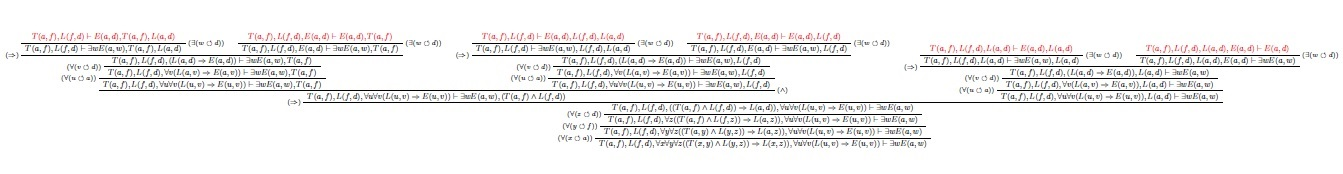
\includegraphics[width=24cm]{figures/RNFa}
	\end{turn}
	\caption[1 melleklet]{1. Példa bizonyítási fája}
	\label{fig-melleklet1}
\end{figure}

\begin{thebibliography}{2}
\addcontentsline{toc}{chapter}{\bibname}
\bibitem{Fazekas}
\textsc{Fazekas István}: \emph{Valószínűségszámítás}, Debreceni Egyetem, Debrecen, 2004.
\bibitem{Tomacs}
\textsc{Tómács Tibor}: \emph{A valószínűségszámítás alapjai}, Líceum Kiadó, Eger, 2005.
\bibitem{VartereszI1} \textsc{Várterész Magdolna}: \emph{Az informatika logika alapjai előadások}, 2006/07-es tanév 1.félév, \url{http://users.atw.hu/de-mi/index.php?r=file/download\&id=219},  Letöltve: 2019 március 12.-én
\end{thebibliography}
\chapter{Adatbázis ábra}
\centering
\includepdf{Hephaistos.pdf}

% Ide lehet szkennelt dokumentumot, dokumentumokat beszúrni
%\includepdf{}

\end{document}